\begin{frame}
	\frametitle{Signal \& Background Modelling}
	\vspace{15pt}
	\cleft{.4}
	%\vspace{10pt}
	
     Signal:
	\li{``Flat'' W' signal samples are reweighted to a desired \wprime pole mass. }
	\vspace{8pt}
	\hspace{10pt}\includegraphics[width=.9\linewidth]{plots/FEYNMAN/ExamplesUnboxed.png}
	\cright{.3}
	\vspace{10pt}
	 \includegraphics[width=\linewidth]{plots/SignalTemplates_truth.eps}
	\cright{.3}
	\vspace{10pt}
	 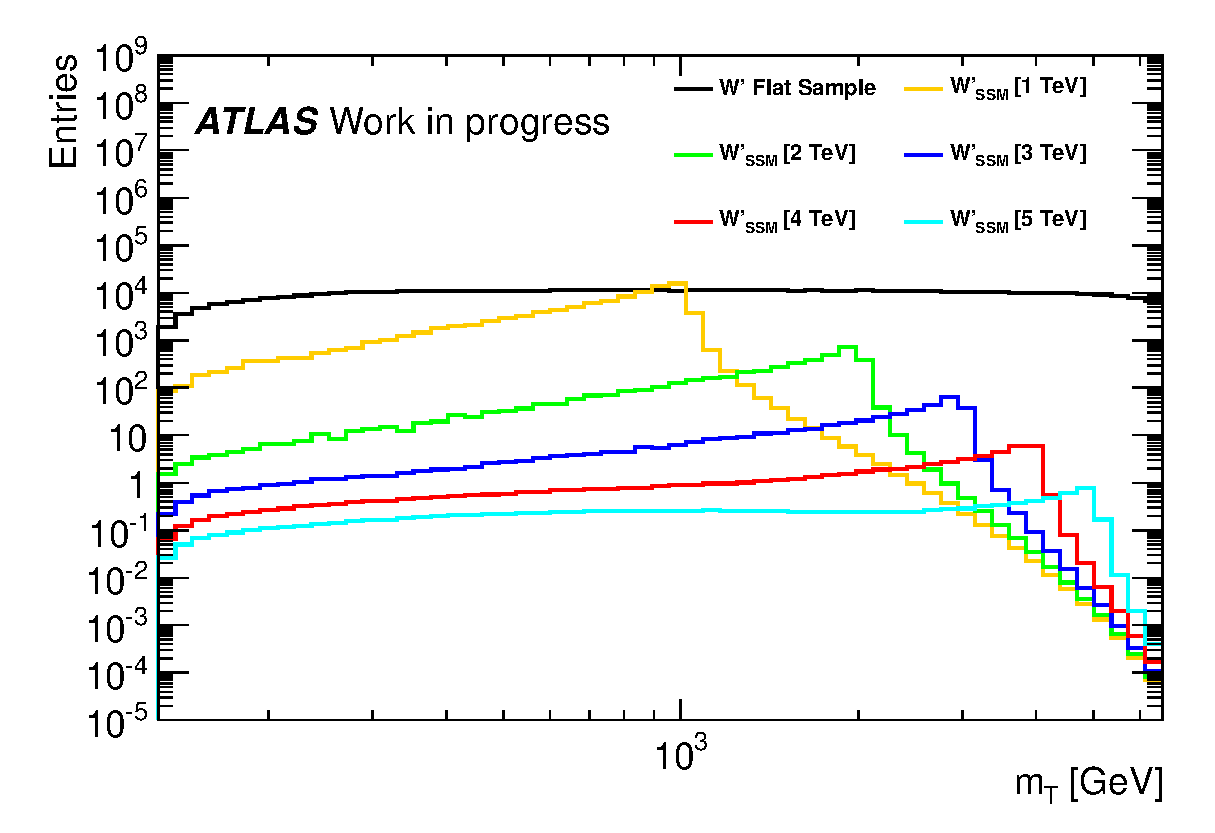
\includegraphics[width=\linewidth]{plots/SignalTemplates.eps}			
	\cend
	\vspace{5pt}
	\cleft{.6}
	Backgrounds:
	\li{Charged Current Drell-Yan $W \rightarrow e \nu$\ {\color{ATLASBlue}(mass-binned)}. \\{\footnotesize This is the \underline{dominant} background}}
	\li{Neutral Current Drell-Yan $Z \rightarrow \ell \ell$ {\color{ATLASBlue}(mass-binned)}. }
	\li{Top ($t\bar{t}$ \& single top) {\color{ATLASBlue}(inclusive + fit)}.}
	\li{Diboson {\color{ATLASBlue}(inclusive + fit)}.}
	
	\li{Multijet background {\color{ATLASBlue}(data-driven 	method + fit)}.}
	\cright{.4}
	
     
   	\includegraphics[width=.9\linewidth]{plots/h_signal_electron_mt_CCDYplus.eps}
   
     
    
   \cend

\end{frame}		